\section{Second application: changing the construction order}
\label{main:next}

The first application replaced one link. The second demonstrates the other move of the design procedure: changing the order in which the links are constructed, which redistributes guarantees and obligations among them. A connected source can still lead to interruptions at the machine. If obstacles divide the robot's safe postures into separate families, a tool path that passes between their regions forces sheet switches, by the same counting argument, and which link fixes that count depends on the construction order. Every reviewed slicer constructs the tool path first. Geometry-first slicing fixes ${\vect{x}}=\Phi\circ{\vect{\upxi}}$, which certifies the occupation measure through $\Phi$, and then seeks a lift ${\vect{q}}=\Psi_{\mathrm{g}}[{\vect{x}}]$ that follows it. Robot-aware methods do plan with machine constraints, but they take a geometric path or geometric elements as input \cite{chalvin2020layer,schmitz2021robot,zhang2021singularity,huang2018choreo}, so obstacles, singularities, and posture changes are resolved for a geometry that is already fixed. Reversing the order is not a permutation of the same maps: $\Psi_{\mathrm{g}}$ lifts a prescribed tool path, whereas a machine-first construction needs a new map $\Psi_{\mathrm{k}}\colon\Xs\to\Qfree$ from the source into admissible configurations, and derives the tool path through forward kinematics (FK; Figure~\ref{fig:kin-order}):
\begin{equation}
  \label{eq:kinematicsfirst}
  {\vect{q}}=\Psi_{\mathrm{k}}\circ{\vect{\upxi}},\qquad {\vect{x}}=\FK\circ {\vect{q}},
\end{equation}
where $\Qfree\subseteq\Qs$ is the set of admissible configurations (within joint limits and free of collisions) and $\FK\colon\Qs\to\mathbb R^3$ returns the tool position. Guarantees and obligations trade places. Static feasibility holds by construction, while coverage and the prescribed occupation measure, ${\vect{x}}_\#\lambda^1=\mu_\Omega$, which geometry-first obtains from $\Phi$, become obligations. Configuration-first coverage exists in robotics: Yang et~al.\ \cite{yang2020coverage} plan coverage through configuration-space cells to minimise discontinuities. The framework adds the prescribed deposition measure and the link to source decomposition.

\begin{figure}[tbp]
  \centering
  \begin{minipage}[t]{0.48\textwidth}
    \centering
    \begin{tikzcd}[column sep=1.8cm, row sep=1.1cm, ampersand replacement=\&]
      \vect{\upxi} \arrow[r, "{\Phi\circ(\cdot)}"] \arrow[dr, dashed, thin] \& \vect{x} \arrow[d, "{\Psi_{\mathrm{g}}[\cdot]}"] \\
      \& \vect{q}
    \end{tikzcd}

    {\small(a) Geometry first\par}
  \end{minipage}\hfill
  \begin{minipage}[t]{0.48\textwidth}
    \centering
    \begin{tikzcd}[column sep=1.8cm, row sep=1.1cm, ampersand replacement=\&]
      \vect{\upxi} \arrow[r, "{\Psi_{\mathrm{k}}\circ(\cdot)}"] \arrow[dr, dashed, thin] \& \vect{q} \arrow[d, "{\FK\circ(\cdot)}"] \\
      \& \vect{x}
    \end{tikzcd}

    {\small(b) Kinematics first\par}
  \end{minipage}

  \caption{The two construction orders. (a) Geometry first: construct the tool path, then lift it to machine motion. (b) Kinematics first: construct admissible machine motion, then derive the tool path through forward kinematics; covering the target $\Omega$ with the prescribed measure remains an obligation. Vertices denote paths. An arrow labelled $f\circ(\cdot)$ applies $f$ pointwise to a path; square brackets denote whole-path input. The dashed diagonals give ${\vect{q}}=\Psi_{\mathrm{g}}[\Phi\circ{\vect{\upxi}}]$ in (a) and ${\vect{x}}=\FK\circ\Psi_{\mathrm{k}}\circ{\vect{\upxi}}$ in (b).}
  \label{fig:kin-order}
\end{figure}

\paragraph{The density obligation.}
\label{sec:kinematics-density}
Let $\Psi_{\mathrm{k}}$ map into a regular submanifold of $\Qfree$ on which $\FK$ is injective in a regular chart, and let $\mu_{\Qs}={\vect{q}}_\#\lambda^1$ be the distribution of deposition time over configurations. The joint path deposits the target exactly when
\[
  \FK_\#\mu_{\Qs}=\mu_\Omega .
\]
Because $\FK$ stretches volume unevenly, a uniform distribution over configurations need not give uniform deposition. Where patches overlap, the target mass is partitioned first and each patch carries its share; multiple preimages must be summed rather than treated as one branch.

\subsection{Posture sheets guide the source split}
\label{sec:kin-sheets}
Once the order is reversed, the robot rather than the target can guide how the source is split, as the part's convexity guided it in the first application (Section~\ref{main:decomposed}). Call the path components of the safe fibre space $\{({\vect{y}},{\vect{q}})\in\Omega\times\Qfree:\FK({\vect{q}})={\vect{y}}\}$ \emph{sheets}. These sheets are related to t-connectivity \cite{wenger1991freeworkspace} and aspects \cite{borrel1986aspects}. A \emph{sheet switch} occurs at a time $t$ where the one-sided limits $({\vect{x}}(t^-),{\vect{q}}(t^-))$ and $({\vect{x}}(t^+),{\vect{q}}(t^+))$ lie in different sheets; a discontinuity within one sheet is not counted. A \emph{posture reset} is a discrete posture change with the flow off; it may be a sheet switch or an in-sheet reset. A continuous stretch of a lifted path stays in one sheet, so a switch is the robot's analogue of a source transition. If one region is reachable only in sheet~1 and another only in sheet~2, every passage of the tool path from the first to the second forces a switch, whatever lift is chosen.

The construction makes the split explicit. (1) Cover $\Omega$ by patches $U_j\subseteq\Omega$, each inside the projection of one sheet. (2) Construct and validate a continuous safe lift of $U_j$ into $\Qfree$ within that sheet. (3) Choose assigned regions $\Omega_j\subseteq U_j$ that cover $\Omega$ with pairwise $\mu_\Omega$-null overlaps, and give piece $j$ its target-mass share $w_j=\mu_\Omega(\Omega_j)>0$ and conditional measure $\mu_\Omega(\,\cdot\mid\Omega_j)$. (4) Traverse each assigned region with its own source piece, using the prepared lift on $U_j$, and visit each piece once.

\begin{proposition}[Sheets force switches; patches attain the minimum]
  \label{prop:sheets-switches}
  Let $\supp\mu_\Omega=\Omega$, where $\supp$ denotes the support of a measure, and let $c$ be the fewest sheets whose projections cover $\Omega$. (i) Every plan with ${\vect{x}}_\#\lambda^1=\mu_\Omega$, finitely many discontinuities, and safe one-sided limits makes at least $c-1$ switches. (ii) If $\Omega$ is covered by $c$ patches $U_j$, with assigned regions $\Omega_j\subseteq U_j$ that partition the target measure as above, and each assigned region is traversed with its conditional measure and time share $w_j$ by a continuous safe lift in one sheet, visiting each assigned region once attains $c-1$. In particular, if two sheets are necessary and two such patches cover $\Omega$, one switch is necessary and sufficient.
\end{proposition}
Appendix~\ref{app:kin-proof} gives the proof. Two distinctions bound the claim. Sheet coverage is not lift existence: a sheet whose projection covers a patch need not supply a continuous lift over it, so the patch lifts are hypotheses to validate. And a counted switch is an event in deposition time, whereas the physical repositioning between postures, with the flow off, is a separate collision-free motion that must be planned and checked. For a fixed path, the same argument fixes the count: with two sheets whose closed projections admit continuous sections, the minimum number of switches equals the number of alternations between the region reached only by the first sheet and the region reached only by the second. A geometry-first slicer inherits this count from its path; a better lift cannot lower it, just as a better order of source pieces cannot lower the number of transitions.

\subsection{A three-link experiment}
\label{sec:kinematics-example}
\paragraph{Setup.}
A planar arm with three revolute joints and unit links deposits on an annular sector among three disk obstacles (Figure~\ref{fig:sheets-3r}(a)). Its safe fibre space is sampled at seven radii; in this sampled availability model, three sheets are necessary and sufficient to cover $\Omega$, so $c=3$. Sampling rules out neither a connection through an unsampled passage nor availability at unsampled radii. Both pipelines use $4^m$ waypoints at orders $m=3,4,5$ and two target densities, uniform and a gradient. \emph{Geometry-first}, our baseline, follows the order-$m$ Hilbert path over the whole chart, solving constrained inverse kinematics at each collocation point, warm-started from the previous solution; when the current sheet fails, it switches to the sheet that stays available longest along the path. \emph{Kinematics-first} follows the construction of Proposition~\ref{prop:sheets-switches}. A one-time preparation places handoff curves between consecutive sheets and stores a certified joint-pose map on each of three patches (Figure~\ref{fig:sheets-3r}(b)). Each request divides the target mass among the assigned regions, traverses each region with its own source piece, and reads joint poses from the stored maps without solving inverse kinematics; consecutive regions are joined at a handoff point, where a posture reset occurs (Figure~\ref{fig:sheets-3r}(d)). The \emph{reset count} is the number of observed discrete posture changes; the \emph{coverage error} is the largest distance from a target grid to the sampled depositing path; the \emph{density error} is the total-variation distance between target shares and waypoint shares on $4\times8$ area bins. Appendix~\ref{app:kin-setup} gives the geometry, sampling, preparation, mass allocation, certification, and timing protocol.

\paragraph{Results.}
Kinematics-first made two sheet switches and no in-sheet resets in all six requests, attaining the bound $c-1=2$ (Table~\ref{tab:sheets-3r-results}). Geometry-first made four sheet switches in every request, the minimum for its fixed Hilbert path in the sampled availability model: the path crosses between regions served by different sheets more often than the cover requires. In two gradient-density requests it also made an additional in-sheet reset, where its warm-started lift lost a branch inside a sheet that still covered the region, an instance of the gap between sheet coverage and lift existence. The excess over $c-1$ is thus a property of the geometry-first path and its lift, not of the solver tolerances, and the reduction to two comes from the sheet-guided split of the source. Coverage errors are comparable and shrink with the order. For uniform density, the geometry-first density error is zero because its waypoints are the Hilbert cell centres, whereas kinematics-first gives each patch a whole number of source columns, and this rounding of mass shares produces its density error; for gradient density the two errors are close. Kinematics-first keeps a sampled clearance of $0.033$ to $0.038$, because its patch maps maximise clearance, while geometry-first's warm-started solutions stay at the imposed margin of $10^{-3}$; its connectors to and from the handoff points add at most $11\%$ of tool travel. After a one-time preparation of $21.0$~s, kinematics-first planned and certified each request in at most $0.17$~s, against $9.3$ to $35.8$~s for geometry-first. The advantage comes from reusing the prepared maps instead of solving inverse kinematics per request, and is not exclusive to kinematics-first construction: a geometry-first planner could also cache inverse maps.

% Written by python -m mapchain tables from results/kinematics/results.json and benchmark.json.
\begin{papertable}
  \begin{papertabular}{llrrrrrrrr}
    \toprule
    & & \multicolumn{2}{c}{Resets} & \multicolumn{2}{c}{Coverage error} & \multicolumn{2}{c}{Density error} & \multicolumn{2}{c}{Planning (s)} \\
    \cmidrule(lr){3-4}\cmidrule(lr){5-6}\cmidrule(lr){7-8}\cmidrule(lr){9-10}
    Density & $m$ & G & K & G & K & G & K & G & K \\
    \midrule
    Uniform & 3 & 4 & 2 & 0.265 & 0.291 & 0.000 & 0.031 & 10.92 & 0.015 \\
    & 4 & 4 & 2 & 0.133 & 0.145 & 0.000 & 0.070 & 18.03 & 0.055 \\
    & 5 & 4 & 2 & 0.066 & 0.069 & 0.000 & 0.029 & 35.79 & 0.168 \\
    \addlinespace
    Gradient & 3 & 4 & 2 & 0.475 & 0.570 & 0.172 & 0.158 & 9.25 & 0.016 \\
    & 4 & 4$+$1 & 2 & 0.250 & 0.217 & 0.043 & 0.068 & 17.04 & 0.055 \\
    & 5 & 4$+$1 & 2 & 0.129 & 0.136 & 0.031 & 0.032 & 29.59 & 0.168 \\
    \bottomrule
  \end{papertabular}
  \caption{Three-link comparison of geometry-first (G) and kinematics-first (K) at $4^m$ waypoints. Resets are observed discrete posture changes: sheet switches, plus in-sheet resets after $+$ where the warm-started lift loses its branch inside a sheet. Coverage error is in target units; density error is total variation of original-waypoint shares on $4\times8$ area bins. Planning time is the median time to plan and certify one request. Kinematics-first also has a one-time preparation of $21.0$~s; the shared fibre analysis ($15.8$~s) is excluded for both.}
  \label{tab:sheets-3r-results}
\end{papertable}


In this example, the change of order placed each obligation where the construction could meet it: density through the source split, up to rounding; clearance in the prepared patch maps; and most of the work in a one-time preparation. These observations hold for one arm, obstacle layout, and implementation, not as general performance guarantees. Admissibility is static, with joint rates and dynamics unchecked, and the posture resets are counted but not planned or certified as physical motions. As in the first application, the forced interruptions are counted by the path components at one link, and a source split matched to those components attains the minimum.

\begin{figure}[H]
  \centering
  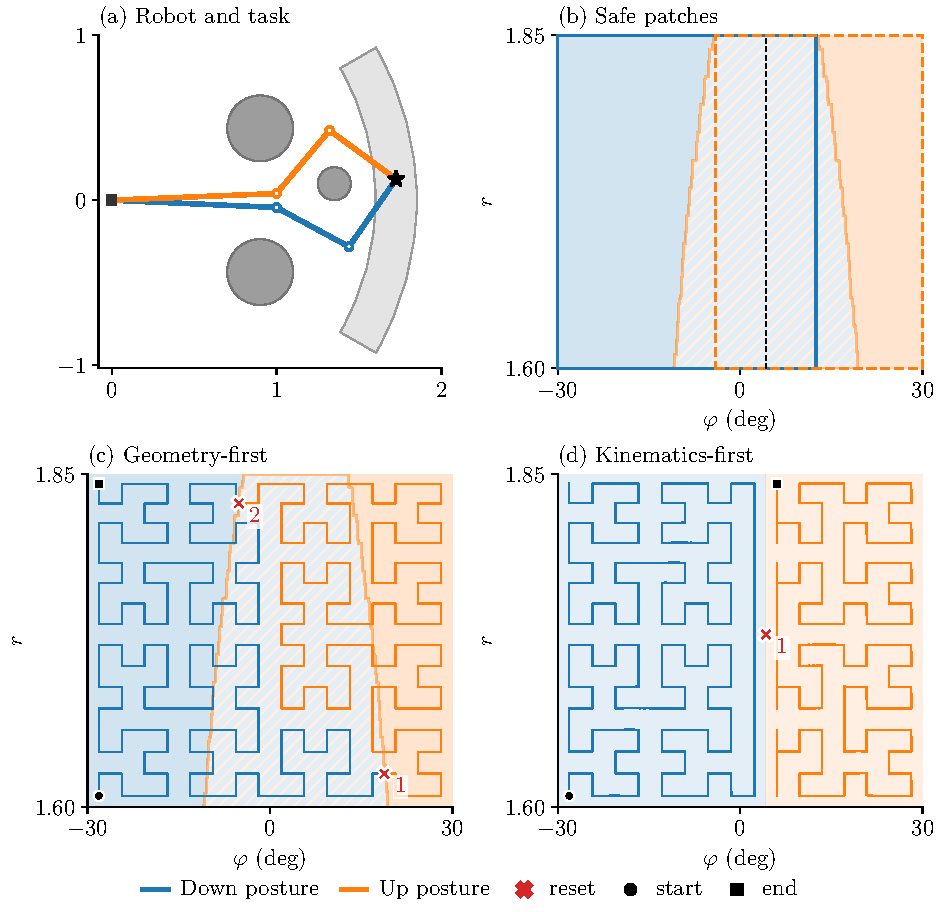
\includegraphics[width=\textwidth]{figures/three_link_posture_comparison.pdf}
  \caption{Three-link experiment at order five with uniform density; colours mark the sheets used. (a) Arm, obstacles, target sector, and the postures available at one tool point. (b) Robot-guided split: sampled availability of the three sheets over the chart, in each sheet's colour where it alone is available and in the mix of the two colours where two are, the certified patch domains $U_j$ (outlines), and the handoff curves (dashed). (c) Geometry-first path, coloured by sheet over the same availability shading, with four sheet switches. (d) Kinematics-first path, shaded by assigned region: each region is completed once, with one sheet switch at each of the two handoff points. Red crosses mark discrete, uncertified posture resets. The certified connectors to and from the handoff points are not drawn.}
  \label{fig:sheets-3r}
\end{figure}
\FloatBarrier
